\documentclass[conference]{IEEEtran}

\usepackage{subfigure,graphicx,url,times,multirow,amsmath,amssymb,algorithm,xspace,epsfig,todonotes,array,caption,color}
\hyphenation{op-tical net-works semi-conduc-tor IEEEtran des-cri-bed}
\usepackage{float}
\usepackage[noend]{algpseudocode}
\usepackage[bookmarks=false]{hyperref}


%\IEEEoverridecommandlockouts

\newcommand{\TODO}[2]{\textcolor{#1}{#2}}
\definecolor{red}{RGB}{255,0,0}
\newcommand{\vect}[1]{\boldsymbol{#1}}
\providecommand{\e}[1]{\ensuremath{\times 10^{#1}}}
\DeclareMathOperator*{\argmax}{arg\,max}

% correct bad hyphenation here
\hyphenation{op-tical net-works semi-conduc-tor}


\begin{document}
%
% paper title
% can use linebreaks \\ within to get better formatting as desired
\title{Neuroevolution for General Video Game Playing}

\author{\IEEEauthorblockN{Spyridon Samothrakis, Diego Perez and Simon Lucas}
\IEEEauthorblockA{School of Computer Science and Electronic Engineering\\
University of Essex, Colchester CO4 3SQ, UK\\
ssamot@essex.ac.uk, dperez@essex.ac.uk, sml@essex.ac.uk}
}


% make the title area
\maketitle


\begin{abstract}
%\boldmath
General Video Game Playing (GVGP) allows for the fair evaluation of algorithms and agents, as it minimiz es the ability of an agent to exploit apriori knowledge in the form of game specific heuristics. In this paper we compare four different, but straightforward, evolutionary algorithms in the new learning stream of the GVGP competition. We show that "crappy results"
\end{abstract}

\IEEEpeerreviewmaketitle

\section{Introduction} \label{sec:intro}

\cite{Perez2014}

\todo[inline]{We have to say somewhere that this is the first time this is done for GVG}

\todo[inline]{I'm not sure if this is up to date with the experiments actually run}

Learning how to act in unknown environments is often termed the ``Reinforcement Learning'' problem\cite{RL}. The problem encapsulates the core of artificial intelligence and has been studied widely under different contexts. Broadly speaking, an agents tries to maximize some long term notion of utility or reward by selecting appropriate actions at each state. Classic RL assumes that state can somehow be identified by the agent in a unique fashion (i.e. the environment has the Markov Property). 

A possible way of attacking the problem in the general sense Neuroevolution\cite{neurocrap}. Neuroevolution adapts adapts the weights of a local or global function approximator (in the form of a neural network) in order to maximize reward. The appeal of neurovolution over traditional gradient-based Reinforcement kerning methods is two fold. First, the gradient in RL problems might be unstable and/or hard to approximate, thus requiring extensive hyper-parameter tuning in order to get any performance. Secondly, the tournament-ranking schemes used by evolutionary approaches are robust to outliers, as they are effectively calculations of medians rather than means. Thirdly, classic RL algorithms (at least their critic-only versions~\cite{jakollacrap} can be greatly impacted by the lack of a perfect markov state. Sensor aliasing is a known and common problem in RL under function approximation. 

On the other hand the lack of direct gradient information limits the possible size of the parameters of the function approximator to be evolved. If provided with the correct setup and hyperparameters, RL algorithms might be able to perform at superhuman level in a number of hard problems. 

In practical terms, research into RL has often been coupled with the use of strong heuristics. General Game Playing allows for completely arbitrary games, making the easy application of temporal based methods non-trivial. On the other hand, modern evolutionary algorithms require minimum fine-tuning and can help greatly with providing a great baseline. In this paper we perform experiments using evolutionary algorithms to learn actors in the following setup. 

\begin{itemize}
\item CMA-ES using e-greedy policy and linear function approximator 
\item CMA-ES using e-gredy policy and neural network
\item CMA-ES using softmax policy and a linear function approximator
\item CMA-ES using softmax policy and a neural network
\end{itemize}

We will see specifics of this setup later. In order to make this research easy to replicate and interesting in its own right, the environmental substrate is provided by a the new track of the General Game Playing AI Competition. We evaluate our players in this setup. 


The paper is structured as follows: blah
 
\section{Related Research} \label{sec:lit}


\todo[inline]{Everything is so well documented}

\todo[inline]{Include here definitions of GGP, GVGP, first attempts. Also GVGAI competition with the planning track (2014)}

\section{The GVGAI Framework} \label{sec:framework}

This section describes the framework and games employed in this research.


\subsection{The framework} \label{ssec:framework}

The General Video Game Playing competition and framework (GVG-AI) is build upon VGDL (Video Game Description Language), a framework designed by Ebner et al.~\cite{Ebner2013} and developed by Tom Schaul~\cite{schaul2013pyvgdl} for GVGP in Python (\textit{py-vgdl}). In VGDL, \textit{objects} interact in a two-dimensional rectangular space, with associated coordinates, and the ability of interact (collide) with each other. VGDL defines an ontology that allows the generation of real-time games and levels with simple text files.

The GVG-AI framework is a Java port of py-vgdl, re-engineered for the GVG-AI Competition by Perez et al.~\cite{Perez2015}, which exposes an interface that allows the implementation of controllers that must determine the actions of the player (also referred to as the \textit{avatar}). The framework provides a \textit{forward model} and information regarding the state of the game to the controllers. The VGDL definition of the game is, however, not provided, so it is the responsibility of the agent to determine the nature of the game and the actions needed to achieve victory. 


\subsection{Games} \label{ssec:games}

\todo[inline]{Games description}

\todo[inline]{The table with the games is exactly the same...}

\begin{table*}[!t]
\begin{center}
\begin{tabular}{|m{1.4cm}|m{8cm}|m{5cm}|m{1cm}|}
\hline
\textbf{Game}  & \textbf{Description} & \textbf{Score} &  \textbf{Actions} \\ 
\hline
\textbf{Aliens} & Similar to traditional Space Invaders, Aliens features the player (avatar) in the bottom of the screen, shooting upwards at aliens that approach Earth, who also shoot back at the avatar. The player loses if any alien touches it, and wins if all aliens are eliminated. & \begin{list}{$\bullet$}{\leftmargin=2pt \itemindent=0em} \item $1$ point is awarded for each alien or protective structure destroyed by the avatar. \item $-1$ point is given if the player is hit. \end{list}  & LEFT, RIGHT, USE.\\
\hline
\textbf{Boulderdash} & The avatar must dig in a cave to find at least $10$ diamonds, with the aid of a shovel, before exiting through a door. Some heavy rocks may fall while digging, killing the player if it is hit from above. There are enemies in the cave that might kill the player, but if two different enemies collide, a new diamond is spawned.& \begin{list}{$\bullet$}{\leftmargin=2pt \itemindent=0em} \item $2$ points are awarded for each diamond collected, and $1$ point every time a new diamond is spawned. \item $-1$ point is given if the avatar is killed by a rock or an enemy. \end{list} & LEFT, RIGHT, UP, DOWN, USE.\\
\hline
\textbf{Butterflies} & The avatar must capture butterflies that move randomly around the level. If a butterfly touches a cocoon, more butterflies are spawned. The player wins if it collects all butterflies, but loses if all cocoons are opened. & \begin{list}{$\bullet$}{\leftmargin=2pt \itemindent=0em} \item $2$ points are awarded for each butterfly captured. \end{list} & LEFT, RIGHT, UP, DOWN.\\
\hline
\textbf{Chase} & The avatar must chase and kill scared goats that flee from the player. If a goat finds another goat's corpse, it becomes angry and chases the player. The player wins if all scared goats are dead, but it loses if is hit by an angry goat. & \begin{list}{$\bullet$}{\leftmargin=2pt \itemindent=0em} \item $1$ point for killing a goat. \item $-1$ point for being hit by an angry goat. \end{list} & LEFT, RIGHT, UP, DOWN.\\
\hline
\textbf{Frogs} & The avatar is a frog that must cross a road, full of tracks, and a river, only traversable by logs, to reach a goal.  The player wins if the goal is reached, but loses if it is hit by a truck or falls into the water. & \begin{list}{$\bullet$}{\leftmargin=2pt \itemindent=0em} \item $1$ point for reaching the goal. \item $-2$ points for being hit by a truck. \end{list} &  LEFT, RIGHT, UP, DOWN. \\
\hline
\textbf{Missile Command} & The avatar must shoot at several missiles that fall from the sky, before they reach the cities they are directed towards. The player wins if it is able to save at least one city, and loses if all cities are hit. &  \begin{list}{$\bullet$}{\leftmargin=2pt \itemindent=0em} \item $2$ points are given for destroying a missile. \item $-1$ point for each city hit. \end{list} & LEFT, RIGHT, UP, DOWN, USE.\\
\hline
\textbf{Portals} & The avatar must find the goal while avoiding lasers that kill him. There are many portals that teleport the player from one location to another. The player wins if the goal is reached, and loses if killed by a laser.& \begin{list}{$\bullet$}{\leftmargin=2pt \itemindent=0em} \item $1$ point is given for reaching the goal. \end{list} & LEFT, RIGHT, UP, DOWN.\\
\hline
\textbf{Sokoban} & The avatar must push boxes so they fall into holes. The player wins if all boxes are made to disappear, and loses when the timer runs out. & \begin{list}{$\bullet$}{\leftmargin=2pt \itemindent=0em} \item $1$ point is given for each box pushed into a hole. \end{list} & LEFT, RIGHT, UP, DOWN.\\
\hline
\textbf{Survive Zombies} & The avatar must stay alive while being attacked by spawned zombies. It may collect honey, dropped by bees, in order to avoid being killed by zombies. The player wins if the timer runs out, and loses if hit by a zombie while having no honey (otherwise, the zombie dies).& \begin{list}{$\bullet$}{\leftmargin=2pt \itemindent=0em} \item $1$ point is given for collecting one piece of honey, and also for killing a zombie. \item $-1$ point if the avatar is killed, or it falls into the zombie spawn point. \end{list} & LEFT, RIGHT, UP, DOWN.\\
\hline
\textbf{Zelda} & The avatar must find a key in a maze to open a door and exit. The player is also equipped with a sword to kill enemies existing in the maze. The player wins if it exits the maze, and loses if it is hit by an enemy. & \begin{list}{$\bullet$}{\leftmargin=2pt \itemindent=0em} \item $2$ points for killing an enemy, $1$ for collecting the key, and another point for reaching the door with it. \item $-1$ point if the avatar is killed. \end{list} & LEFT, RIGHT, UP, DOWN, USE. \\
\hline
\end{tabular}
\caption{Games in the training set of the GVGAI Competition, employed in the experiments of this paper.}
\label{tab:games}
\end{center}
\end{table*}

\todo[inline]{Maybe I can put a different picture here, not to be repetitive with last CIG.}

% \begin{figure*}[!t]
% \begin{center}
% 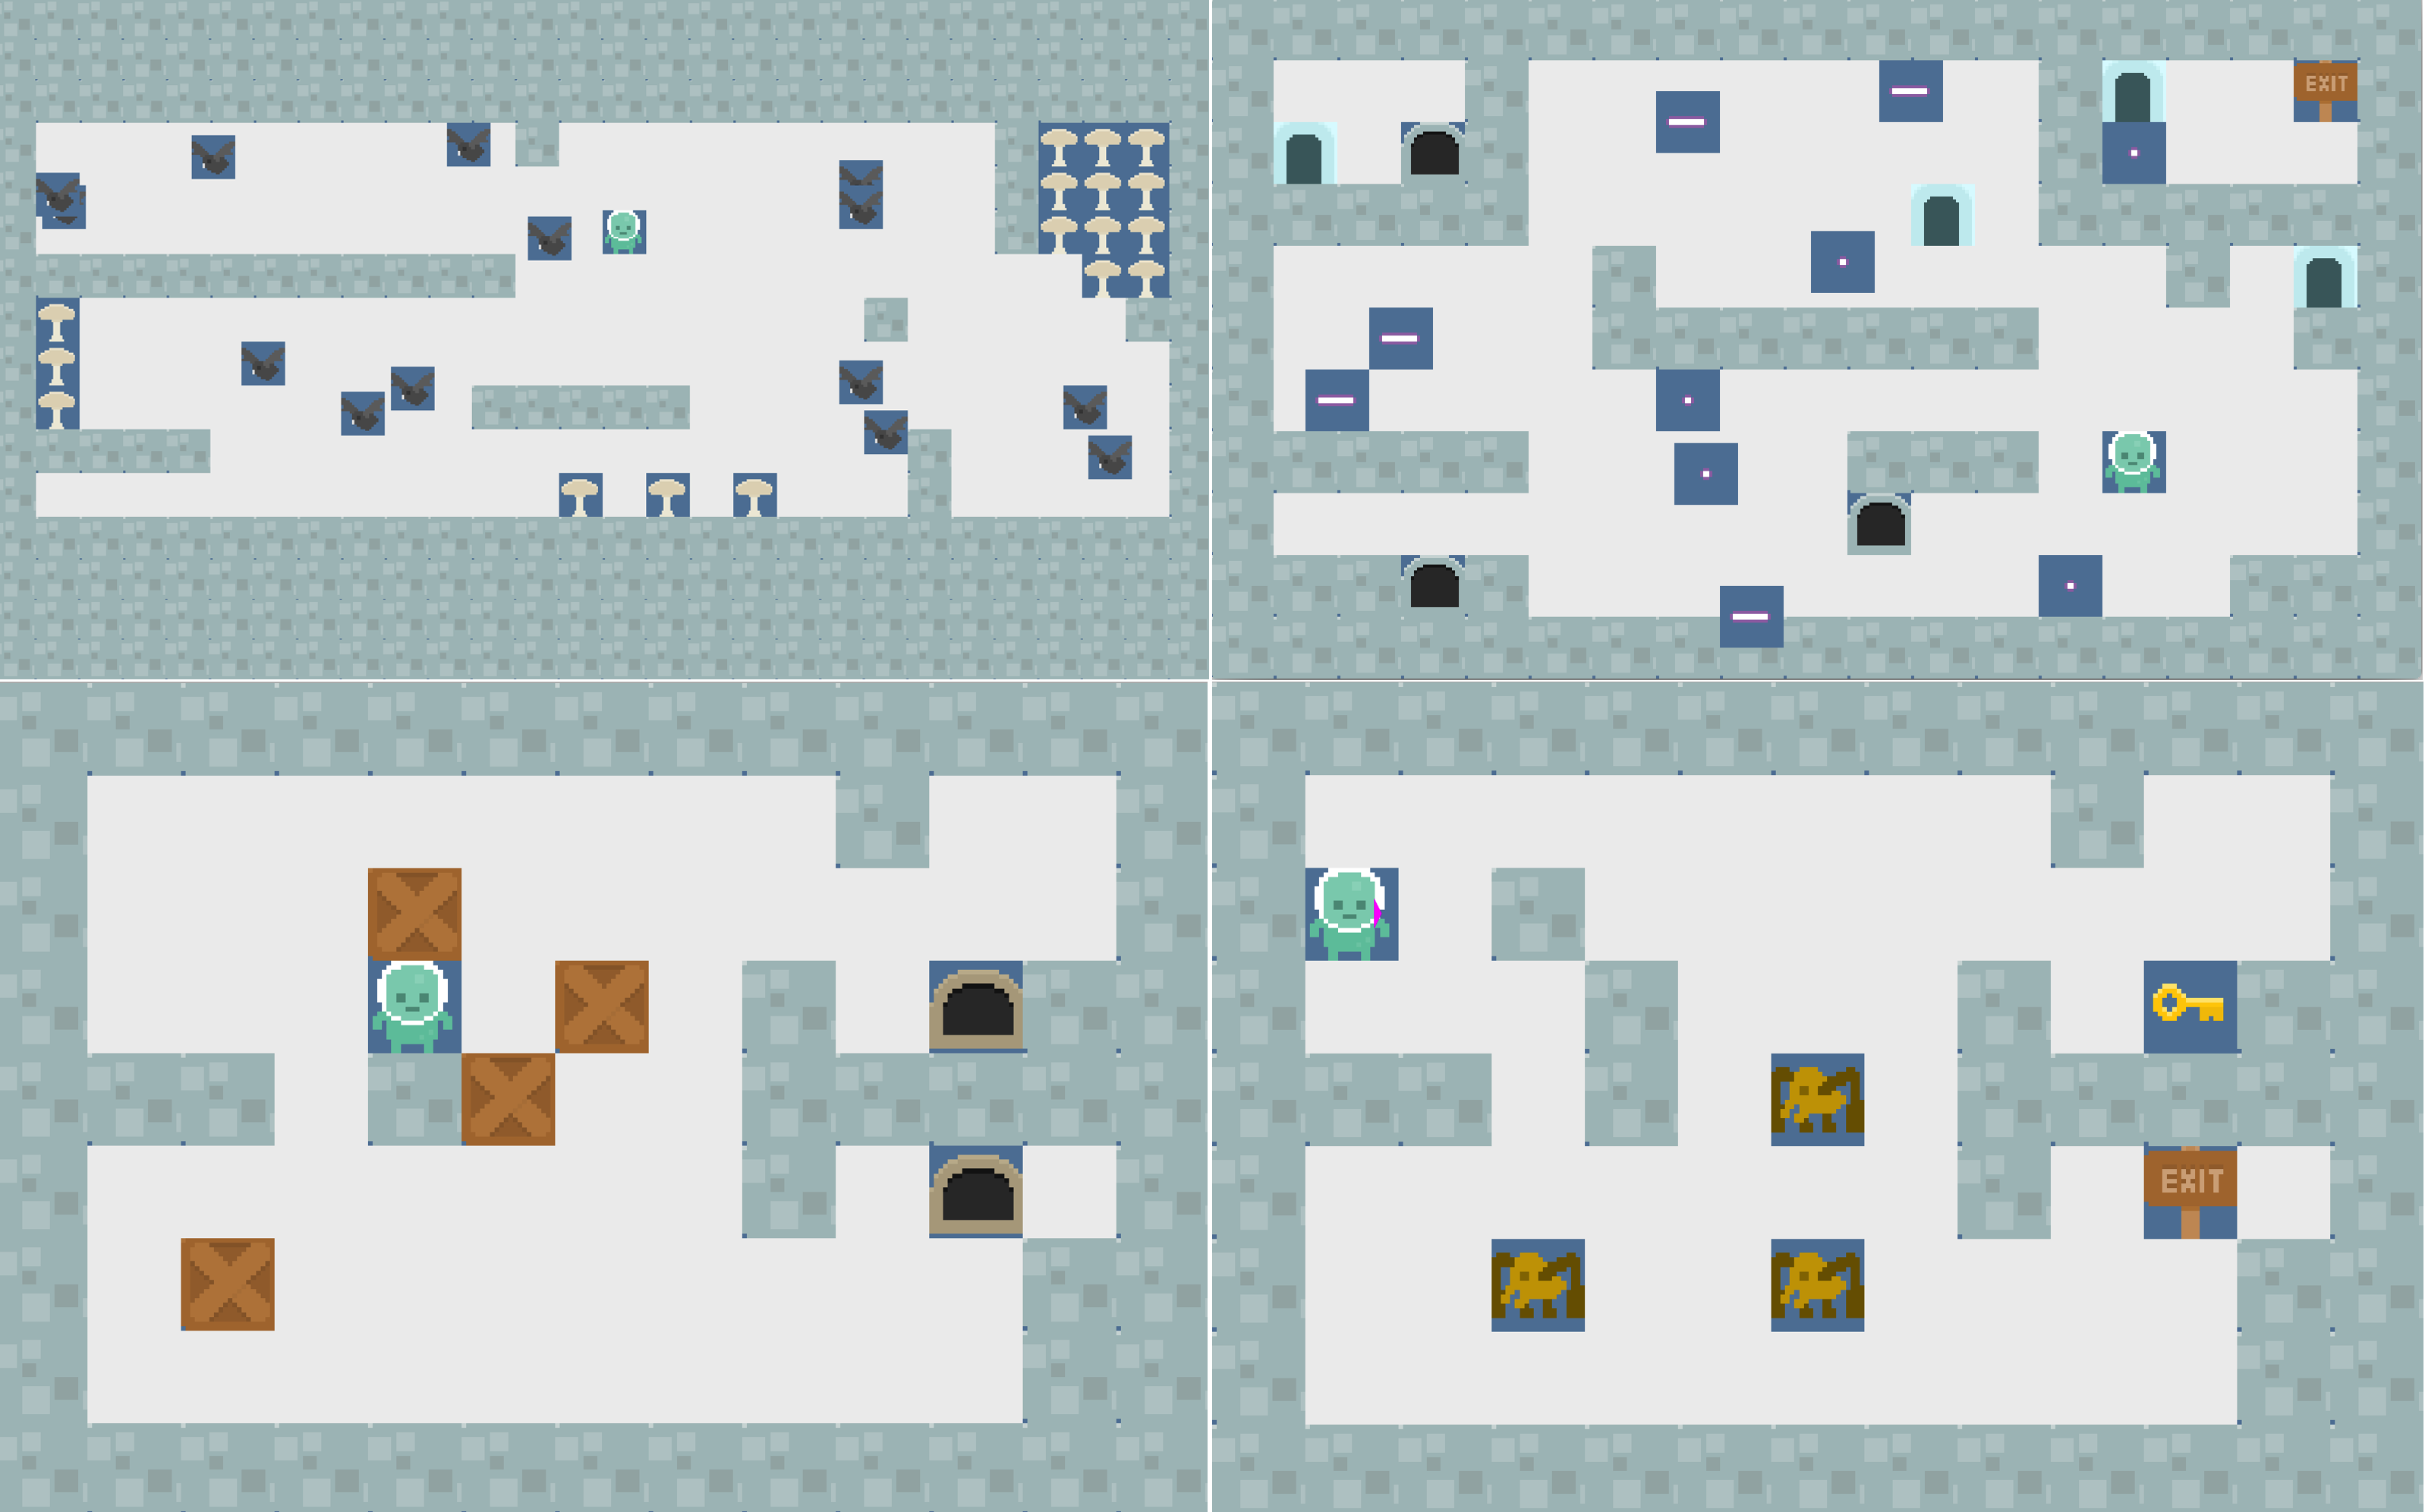
\includegraphics[width=1.8\columnwidth]{img/games}
% \end{center}
% \caption{Four of the ten training set games: from top to bottom, left to right, \textit{Boulderdash}, \textit{Survive Zombies}, \textit{Aliens} and \textit{Frogs}.}
% \label{fig:games}
% \end{figure*}




\section{Background} \label{sec:fastEvo}

\todo[inline]{Everything is so powerful}


\subsection{Approaches} \label{sec:fastEvoMem}

\todo[inline]{Everything is so cool}


\section{Experiments} \label{sec:exp}

\todo[inline]{Everything took so long}



\section{Conclusions} \label{sec:conc}

\todo[inline]{Everything is so pretty}

% use section* for acknowledgement
 
\section*{Acknowledgment}


\noindent This work was supported by EPSRC grant EP/H048588/1.

\bibliographystyle{IEEEtran} 
\bibliography{biblio}


% that's all folks
\end{document}


